\documentclass{ximera}

\title{From Curves to Surfaces: Understanding Directional Derivatives}
\author{Zack Reed}

\begin{document}
\begin{abstract}
We extend our understanding of derivatives from single-variable curves to multivariable surfaces by exploring how cutting through a surface's domain creates curves we can differentiate.
\end{abstract}
\maketitle

\section*{From Single Variables to Multiple Variables}

In single-variable calculus, we studied functions $f(x)$ that created curves in 2D space. Now we're moving to functions $f(x,y)$ that create surfaces in 3D space. This requires some extra care when taking derivatives, which currently only make sense with respect to curves.

\section*{Recap: Derivatives of Curves}

Right now our methods for differentiating utilize curves in space. We will first use this to introduce the idea of a derivative at a point on a surface in a certain direction, and then will finish with a more general method for computing these derivatives.

The following video sets up the context for the problem below:
\begin{center}
\youtube{6ErX1VqK05Q}
\end{center}

\begin{problem}

We've extensively examined the race between Torty and Harry, as seen in the following applet:

\begin{center}
\geogebra{yzxdk5uw}{844}{629}
\end{center}

Now that we have some experience with multivariable functions, we can actually describe the racetrack in greater detail. 

The ``hill'' is the surface from the function $z = f(x,y) = xy^2$. The racetrack is the curve that follows the hill, specifically along the unit circle in the $xy$-plane. The unit circle is parametrized by $\vec{r}(t) = \langle \cos(t), \sin(t) \rangle$, so we get the vector function (for Harry):

$$\vec{C}(t) = \langle \cos(t), \sin(t), f(\cos(t), \sin(t)) \rangle = \langle \cos(t), \sin(t), \cos(t) \sin^2(t) \rangle$$

Mark all of the following statements that are true:

\begin{selectAll}
\choice[correct]{The racetrack is a curve on the surface defined by $z = f(x,y)$.}
\choice{The racetrack is a surface defined by $z = f(x,y)$.}
\choice[correct]{The racetrack can be represented as a vector function $\vec{C}(t)$.}
\choice{The racetrack cannot be represented as a vector function because it is on a surface.}
\choice[correct]{The racetrack is created by following a path through the domain of $f(x,y)$.}
\choice{The racetrack is created by following a path on the surface of $f(x,y)$.}
\end{selectAll}

Moving forward, we'll often need to check whether a calculation or object is in the domain of the function, or is a vector or other quantity in the space in which the surface lives. The output curve lives in 3D space on the surface, but we create it by following a path through the 2D domain.

\end{problem}

This process of creating a curve on a surface by isolating a path through the domain is key to initially understanding derivatives of multivariable functions.


\section*{Direction of Derivatives: Cutting through the Domain}

Consider a function $z = f(x,y)$. The domain (input space) is the $xy$-plane, and the output is a height $z$ above each point $(x,y)$.

The plot below gives an example line cutting through the domain of a function.

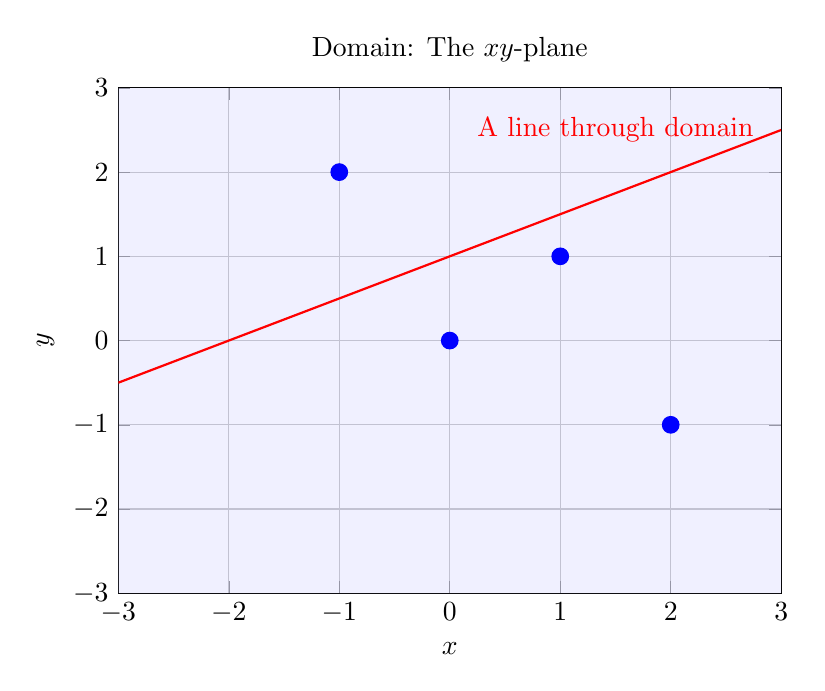
\begin{tikzpicture}
\begin{axis}[
    width=10cm,
    height=8cm,
    xlabel=$x$,
    ylabel=$y$,
    xmin=-3, xmax=3,
    ymin=-3, ymax=3,
    grid=major,
    title={Domain: The $xy$-plane}
]
% Draw the domain as a filled region
\addplot[fill=blue!20, opacity=0.3] coordinates {(-3,-3) (3,-3) (3,3) (-3,3) (-3,-3)};

% Show a few sample points
\addplot[only marks, mark=*, mark size=3pt, blue] coordinates {(0,0) (1,1) (-1,2) (2,-1)};

% Draw a line through the domain
\addplot[thick, red, domain=-3:3] {0.5*x + 1};
\node[red] at (axis cs:1.5,2.5) {A line through domain};

\end{axis}
\end{tikzpicture}


\section*{Creating Curves from Surfaces}

When we follow a line through the domain of a function and look at the corresponding function values, we get a curve in 3D space!

If our line through the domain is parametrized as:
$$\vec{r}(t) = \langle x(t), y(t) \rangle$$

Then the resulting curve in 3D space is:
$$\vec{C}(t) = \langle x(t), y(t), f(x(t), y(t)) \rangle$$

This is just like the creation of the racetrack earlier. The main point is that at each $(x,y)$ pair along the line, we find the height $z = f(x,y)$ to get the full 3D point.

The following video discusses the main idea:

\begin{center}
\youtube{2Lbl8rH7EAs}
\end{center}

Let's practice generating a curve from a surface before moving on.

\begin{problem}
Consider the hill of the Torty Harry Race, $h(x,y) = xy^2$. Lines through the domain create curves on the surface, as see in the following applet:

\begin{expandable}{stuff}{GeoGebra Instructions}
 If you click and drag on the blued dot, you move the point in the domain at which the function is evaluated. There is a direction vector coming from the point. Moving the red dot will change the direction of the vector.

 The direction creates a line through the domain, and on the right you can see the resulting curve cut through the hill along that line.
\end{expandable}

\begin{center}
\geogebra{qebmdea2}{639}{329}
\end{center}

Let's look at a specific point in the domain, and a direction in which to move. 

Our function is $f(x,y) = xy^2$. We will take a derivative at the point $(0,1)$ in the direction given by $\vec{u} = \langle \frac{\sqrt{2}}{2}, \frac{\sqrt{2}}{2} \rangle$. This selection of a point is the same as picking a point for the derivative in single-variable calculus, the addition of a direction for the derivative is new, and is important for our new context of having multiple input variables.

The direction gives us a line in the domain. The specific line given by $x(t) = \answer[tolerance=.1]{\frac{\sqrt{2}}{2}}t+ \answer{0}$, $y(t) = \frac{\sqrt{2}}{2}t + \answer{1}$.

We now need to make a curve in 3D space resulting from evaluation of the function along this line. The height of our point $(0,1)$ on the surface is $f(0,1) = 0 \cdot 1^2 = \answer{0}$.

Since the height of our curve is given by $f(x(t), y(t))$, we have (answer with a formula in terms of $t$):

$$f(x(t), y(t)) = f\left(\frac{\sqrt{2}}{2}t, \frac{\sqrt{2}}{2}t + 1\right) = \left(\frac{\sqrt{2}}{2}t\right)\left(\frac{\sqrt{2}}{2}t + 1\right)^2$$

This simplifies to $\answer[tolerance=.1]{\frac{\sqrt{2}}{4}}t^3 + \answer[tolerance=.1]{1}t^2 + \answer[tolerance=.1]{\frac{\sqrt{2}}{2}}t$.

The resulting curve in 3D space is $\vec{C}(t) = \left\langle \frac{\sqrt{2}}{2}t, \frac{\sqrt{2}}{2}t + 1, \answer[tolerance=.1]{\frac{\sqrt{2}}{4}}t^3 + \answer[tolerance=.1]{1}t^2 + \answer[tolerance=.1]{\frac{\sqrt{2}}{2}}t \right\rangle$.

\begin{feedback}
Since $f(x,y) = xy^2$ and we want the derivative at $(0,1)$ in the direction $\vec{u} = \langle \frac{\sqrt{2}}{2}, \frac{\sqrt{2}}{2} \rangle$, we can parametrize the line through the domain as:
$$x(t) = \frac{\sqrt{2}}{2} \cdot t + 0 = \frac{\sqrt{2}}{2}t$$
$$y(t) = \frac{\sqrt{2}}{2} \cdot t + 1 = \frac{\sqrt{2}}{2}t + 1$$

Evaluating the function along this line:
$$f(x(t), y(t)) = f\left(\frac{\sqrt{2}}{2}t, \frac{\sqrt{2}}{2}t + 1\right) = \left(\frac{\sqrt{2}}{2}t\right)\left(\frac{\sqrt{2}}{2}t + 1\right)^2$$
\end{feedback}
\end{problem}

\section*{Derivatives Along These Curves}

Now we can take derivatives of these curves just like we did in vector calculus! These are called \emph{directional derivatives} because they give the rate of change of the function at certain points, in a certain direction.

We will quickly develop simpler ways to compute these derivatives, but we will start by directly differentiating the underlying curves to get an intuition about what the derivatives are telling us.

For the curve $\vec{C}(t) = \langle x(t), y(t), f(x(t), y(t)) \rangle$:

$$\vec{C}'(t) = \left\langle \frac{dx}{dt}, \frac{dy}{dt}, \frac{df}{dt} \right\rangle$$

Let's see what this directional derivative would be with our hill example.

\begin{problem}
For the function $f(x,y) = xy^2$ at the point $(0,1)$ in the direction $\vec{u} = \langle \frac{\sqrt{2}}{2}, \frac{\sqrt{2}}{2} \rangle$, we found the curve:
$$\vec{C}(t) = \left\langle \frac{\sqrt{2}}{2}t, \frac{\sqrt{2}}{2}t + 1, \frac{\sqrt{2}}{4}t^3 + 1\cdot t^2 + \frac{\sqrt{2}}{2}t \right\rangle$$

We might want to know the following question which directly extends our single-variable derivative concept: 

``If we stand at the point $(0,1)$ on the surface and move in the direction $\vec{u}$, how fast does the hill height change?''

Notice that we are explicitly asking about the rate of change only of the height of the hill. 

Since the output of multivariable functions is a single variable, the derivatives tell us only how that output variable changes. All other information is given to us, and relates to the input variables.

Let's answer the question explicitly since we have the curve.

The height of the hill along the curve is given by the third component of $\vec{C}(t)$, which is $f(x(t), y(t)) = \frac{\sqrt{2}}{4}t^3 + 1\cdot t^2 + \frac{\sqrt{2}}{2}t$.

Therefore, the rate of change of the hill height as we move along the curve is given by:
$$\frac{d}{dt}[f(x(t), y(t))] = \frac{d}{dt}\left[\frac{\sqrt{2}}{4}t^3 + 1\cdot t^2 + \frac{\sqrt{2}}{2}t\right] = \answer[tolerance=.1]{\frac{3\sqrt{2}}{4}}t^2 + \answer[tolerance=.1]{2}t + \answer[tolerance=.1]{\frac{\sqrt{2}}{2}}$$

At our point of interest $(0,1)$, $t = 0$, so the rate of change of the hill height at $(0,1)$ in the direction $\vec{u}$ is:
$$\frac{d}{dt}[f(x(t), y(t))]\bigg|_{t=0} = \answer[tolerance=.1]{\frac{\sqrt{2}}{2}}$$

This means:

\begin{multipleChoice}
\choice{The hill height does not change as we move in the direction $\vec{u}$ from the point $(0,1)$.}
\choice[correct]{The hill height increases at a rate of $\frac{\sqrt{2}}{2}$ units of height per unit of movement in the direction $\vec{u}$ from the point $(0,1)$.}
\choice{The hill height decreases at a rate of $\frac{\sqrt{2}}{2}$ units of height per unit of movement in the direction $\vec{u}$ from the point $(0,1)$.}
\choice{The hill height increases at a rate of $\frac{\sqrt{2}}{2}$ units of height per unit of movement in the $x$ direction from the point $(0,1)$.}
\choice{The hill height increases at a rate of $\frac{\sqrt{2}}{2}$ units of height per unit of movement in the $y$ direction from the point $(0,1)$.}
\end{multipleChoice}
\end{problem}

Let's practice computing these derivatives directly from the curves to get the main idea, and then we will introduce easier and more general methods for computing these same derivatives.

\begin{problem}
Compute the following directional derivatives and answer the provided questions.
\begin{enumerate}
  \item  $f(x,y) = x^2 + y^2$ at the point $(1,2)$ in the direction $\vec{u} = \langle -0.15, 0.989 \rangle$.
  
  Step 1: Parametrize the line through the domain:
  $$x(t) = \answer[tolerance=.1]{-0.15}t + \answer{1}$$
  $$y(t) = \answer[tolerance=.1]{0.989}t + \answer{2}$$
  Step 2: Create the curve in 3D space:
  $$f(x(t), y(t)) = f(-0.15t + 1, 0.989t + 2) = (-0.15t + 1)^2 + (0.989t + 2)^2$$ 
  $$= \answer[tolerance=.1]{1}t^2 + \answer[tolerance=.1]{3.656}t + \answer{5}$$

  Step 3: Differentiate the height function:
  $$\frac{d}{dt}[f(x(t), y(t))] = \answer[tolerance=.1]{3.656} + \answer[tolerance=.1]{2}t$$

  Step 4: Evaluate at the point of interest. Since we are at $(1,2)$, $t = 0$:
  $$\frac{d}{dt}[f(x(t), y(t))]\bigg|_{t=0} = \answer[tolerance=.1]{3.656}$$

  \item  $f(x,y) = x^2 + y^2$ at the point $(0,0)$ in the direction $\vec{u} = \langle -1/2,\frac{\sqrt{3}}{2} \rangle$.
  
  Step 1: Parametrize the line through the domain:
  $$x(t) = \answer{-\frac{1}{2}}t + \answer{0}$$
  $$y(t) = \answer{\frac{\sqrt{3}}{2}}t + \answer{0}$$
  Step 2: Create the curve in 3D space:
  $$f(x(t), y(t)) = f\left(-\frac{1}{2}t, \frac{\sqrt{3}}{2}t\right) = \left(-\frac{1}{2}t\right)^2 + \left(\frac{\sqrt{3}}{2}t\right)^2 = \answer{t^2}$$

  Step 3: Differentiate the height function:
  $$\frac{d}{dt}[f(x(t), y(t))] = \answer{2t}$$

  Step 4: Evaluate at the point of interest. Since we are at $(0,0)$, $t = 0$:
  $$\frac{d}{dt}[f(x(t), y(t))]\bigg|_{t=0} = \answer{0}$$

  \item  $f(x,y) = \cos(x)\cdot\sin(y)$ at the point $(\frac{\pi}{2}, \frac{\pi}{2})$ in the direction $\vec{u} = \langle 0.53, 0.85 \rangle$.
  
  Step 1: Parametrize the line through the domain:
  $$x(t) = \answer[tolerance=.1]{0.53}t + \answer{\frac{\pi}{2}}$$
  $$y(t) = \answer[tolerance=.1]{0.85}t + \answer{\frac{\pi}{2}}$$

  Step 2: Create the curve in 3D space:
  $$f(x(t), y(t)) = f(0.53t + \frac{\pi}{2}, 0.85t + \frac{\pi}{2}) = \cos(0.53t + \frac{\pi}{2}) \cdot \sin(0.85t + \frac{\pi}{2}) = -\sin(0.53t)\cos(0.85t)$$

  Step 3: Differentiate the height function:
  $$\frac{d}{dt}[f(x(t), y(t))] = -0.53\cos(0.53t)\cos(0.85t) + 0.85\sin(0.53t)\sin(0.85t)$$

  Step 4: Evaluate at the point of interest. Since we are at $(\pi/2, \pi/2)$, $t = 0$:
  $$\frac{d}{dt}[f(x(t), y(t))]\bigg|_{t=0} = \answer[tolerance=.1]{-0.53}$$

\end{enumerate}

\end{problem}

\begin{problem}
Which of the following statements is true about the directional derivatives computed above?
\begin{multipleChoice}
\choice{Directoinal derivatives give the rate of change of all input variables.}
\choice[correct]{Directional derivatives give the rate of change of the output variable in a certain direction through the domain.}
\choice{Directional derivatives give the rate of change of the input variables in a certain direction through the domain.}
\choice{Directional derivatives give the rate of change of all output variables.}
\end{multipleChoice}

\begin{feedback}
Directional derivatives only give the rate of change of the output variable (the function value) as we move in a certain direction through the domain. The input variables are given to us by the parametrization of the line through the domain.
\end{feedback}
\end{problem}

\end{document}